
\documentclass[11pt]{article}
\usepackage{amsmath, amssymb, graphicx, outline, float, cite, color}

%%%%%%%%%%%%%%%%%%%%%%%%%%%%%%%%%%%%%%%%%
% Wenneker Article
% Structure Specification File
% Version 1.0 (28/2/17)
%
% This file originates from:
% http://www.LaTeXTemplates.com
%
% Authors:
% Frits Wenneker
% Vel (vel@LaTeXTemplates.com)
%
% License:
% CC BY-NC-SA 3.0 (http://creativecommons.org/licenses/by-nc-sa/3.0/)
%
%%%%%%%%%%%%%%%%%%%%%%%%%%%%%%%%%%%%%%%%%

%----------------------------------------------------------------------------------------
%	PACKAGES AND OTHER DOCUMENT CONFIGURATIONS
%----------------------------------------------------------------------------------------

\usepackage[english]{babel} % English language hyphenation

\usepackage{microtype} % Better typography

\usepackage{amsmath,amsfonts,amsthm} % Math packages for equations

\usepackage[svgnames]{xcolor} % Enabling colors by their 'svgnames'

\usepackage[hang, small, labelfont=bf, up, textfont=it]{caption} % Custom captions under/above tables and figures

\usepackage{booktabs} % Horizontal rules in tables

\usepackage{lastpage} % Used to determine the number of pages in the document (for "Page X of Total")

\usepackage{graphicx} % Required for adding images

\usepackage{enumitem} % Required for customising lists
\setlist{noitemsep} % Remove spacing between bullet/numbered list elements

\usepackage{sectsty} % Enables custom section titles
\allsectionsfont{\usefont{OT1}{phv}{b}{n}} % Change the font of all section commands (Helvetica)

%----------------------------------------------------------------------------------------
%	MARGINS AND SPACING
%----------------------------------------------------------------------------------------

\usepackage{geometry} % Required for adjusting page dimensions

\geometry{
	top=2cm, % Top margin
	bottom=2cm, % Bottom margin
	left=3cm, % Left margin
	right=3cm, % Right margin
	includehead, % Include space for a header
	includefoot, % Include space for a footer
	%showframe, % Uncomment to show how the type block is set on the page
}

\setlength{\columnsep}{7mm} % Column separation width

%----------------------------------------------------------------------------------------
%	FONTS
%----------------------------------------------------------------------------------------

\usepackage[T1]{fontenc} % Output font encoding for international characters
\usepackage[utf8]{inputenc} % Required for inputting international characters

\usepackage{XCharter} % Use the XCharter font

%----------------------------------------------------------------------------------------
%	HEADERS AND FOOTERS
%----------------------------------------------------------------------------------------

\usepackage{fancyhdr} % Needed to define custom headers/footers
\pagestyle{fancy} % Enables the custom headers/footers

\renewcommand{\headrulewidth}{0.0pt} % No header rule
\renewcommand{\footrulewidth}{0.4pt} % Thin footer rule

\renewcommand{\sectionmark}[1]{\markboth{#1}{}} % Removes the section number from the header when \leftmark is used

%\nouppercase\leftmark % Add this to one of the lines below if you want a section title in the header/footer

% Headers
\lhead{} % Left header
\chead{\textit{\thetitle}} % Center header - currently printing the article title
\rhead{} % Right header

% Footers
\lfoot{} % Left footer
\cfoot{} % Center footer
\rfoot{\footnotesize Page \thepage\ of \pageref{LastPage}} % Right footer, "Page 1 of 2"

\fancypagestyle{firstpage}{ % Page style for the first page with the title
	\fancyhf{}
	\renewcommand{\footrulewidth}{0pt} % Suppress footer rule
}

%----------------------------------------------------------------------------------------
%	TITLE SECTION
%----------------------------------------------------------------------------------------

\newcommand{\authorstyle}[1]{{\large\usefont{OT1}{phv}{b}{n}\color{DarkRed}#1}} % Authors style (Helvetica)

\newcommand{\institution}[1]{{\footnotesize\usefont{OT1}{phv}{m}{sl}\color{Black}#1}} % Institutions style (Helvetica)

\usepackage{titling} % Allows custom title configuration


%\newcommand{\HorRule}{\color{DarkGrey}\rule{\linewidth}{1pt}} % Defines the gold horizontal rule
\newcommand{\HorRule}{\color{DarkGoldenrod}\rule{\linewidth}{1pt}} % Defines the gold horizontal rule
 
\pretitle{
	\vspace{-30pt} % Move the entire title section up
	\HorRule\vspace{10pt} % Horizontal rule before the title
	\fontsize{20}{18}\usefont{OT1}{phv}{b}{n}\selectfont % Helvetica
	\color{DarkRed} % Text colour for the title and author(s)
}

\posttitle{\par\vskip 15pt} % Whitespace under the title

\preauthor{} % Anything that will appear before \author is printed

\postauthor{ % Anything that will appear after \author is printed
	\vspace{10pt} % Space before the rule
	\par\HorRule % Horizontal rule after the title
	\vspace{20pt} % Space after the title section
}

%----------------------------------------------------------------------------------------
%	ABSTRACT
%----------------------------------------------------------------------------------------

\usepackage{lettrine} % Package to accentuate the first letter of the text (lettrine)
\usepackage{fix-cm}	% Fixes the height of the lettrine

\newcommand{\initial}[1]{ % Defines the command and style for the lettrine
	\lettrine[lines=3,findent=4pt,nindent=0pt]{% Lettrine takes up 3 lines, the text to the right of it is indented 4pt and further indenting of lines 2+ is stopped
		%\color{DarkRed}% Lettrine colour
		\color{DarkGoldenrod}% Lettrine colour
		{#1}% The letter
	}{}%
}

\usepackage{xstring} % Required for string manipulation

\newcommand{\lettrineabstract}[1]{
	\StrLeft{#1}{1}[\firstletter] % Capture the first letter of the abstract for the lettrine
	\initial{\firstletter}\textbf{\StrGobbleLeft{#1}{1}} % Print the abstract with the first letter as a lettrine and the rest in bold
}

%----------------------------------------------------------------------------------------
%	BIBLIOGRAPHY
%----------------------------------------------------------------------------------------

%\usepackage[backend=bibtex,style=authoryear,natbib=true]{biblatex} % Use the bibtex backend with the authoryear citation style (which resembles APA)

%\addbibresource{example.bib} % The filename of the bibliography

%\usepackage[autostyle=true]{csquotes} % Required to generate language-dependent quotes in the bibliography
 % Specifies the document structure and loads requires packages


\graphicspath{ {Figs/} }

\usepackage[T1]{fontenc}
\usepackage[utf8]{inputenc}
\usepackage{authblk}

%\usepackage[ ]{natbib} 
\newcommand{\tcr} { \textcolor{red} }


% A multiscale model of EMT-mediated cancer reveals 
\title{Multiscale Modeling of the Paradoxical Roles of the Immune System in EMT-Mediated Cancer}
\author{Daniel R. Bergman$^{1}$,
Matthew Karikomi\,$^{1}$,
Qing Nie\,$^{1,2,*}$
and Adam L. MacLean\,$^{3,*}$
}
\affil{
  $^1$Department of Mathematics, University of California, Irvine,  Irvine, CA 92697, USA \\
  $^2$Department of Cell and Developmental Biology, University of California, Irvine, Irvine, CA 92697, USA \\
  $^3$Department of Biological Sciences, University of Southern California, Los Angeles, CA 90089, USA \\
  $^*$Correspondence:  qnie@uci.edu (QN); macleana@usc.edu (ALM).
}

\renewcommand\Authands{ and }

\date{}


\begin{document}
\maketitle


\section*{Abstract}
Preceding tumorigenesis and throughout the lifetime of a tumor, the immune system is engaged in complex sets of interactions in and around the tumor. These are regulated by the tumor microenvironment (TME) in myriad ways. Moreover,  epithelial cell plasticity impacts disease incidence and progression via processes of epithelial-to-mesenchymal transition (EMT).
In turn, both the tumor and the immune system exert substantial influence over the TME in competition to influence the fate of the host. Determining the factors and mechanisms underpinning these complex interactions remains an important task for cancer immunotherapy. We developed a multiscale agent-based model to describe the interplay between three components: the tumor (or pre-tumor cells), the immune system, and EMT.
The model revealed a \tcr{non-monotonic relationship} between the cell cycle times associated with the mesenchymal phenotype and the probability of tumorigenesis, identifying a critical growth rate that maximizes cancer-free survival. In comparison, increasing the immune-evasiveness of the mesenchymal phenotypes always led to poorer prognosis. Moreover, encouraging the TME
towards a pro-EMT state also benefits the tumor. Together, these results indicate that the joint regulation of the TME by the immune system and the tumor itself provides possible targets for future cancer therapies, in particular cancers such as pancreatic cancer in which EMT is speculated to play a role.



%% Basic Introduction (1-2 sentences)
%Preceding tumorigenesis and throughout the lifetime of a tumor, the immune system is engaged in complex sets of interactions in and around the tumor.
%% More Detailed Background (2-3 sentences)
%These are regulated by the tumor microenvironment (TME) in myriad ways. Moreover,  epithelial cell plasticity impacts disease incidence and progression via processes of epithelial-to-mesenchymal transition (EMT).
%In turn, both the tumor and the immune system exert substantial influence over the TME in competition to influence the fate of the host.
%% General Problem (1 sentence)
%Determining the factors and mechanisms underpinning these complex interactions remains an important task for cancer immunotherapy.
%% Summarizing Main Result (1 sentence)
%Here, we seek to understand how interplay between the tumor, the immune system, and EMT can determine the outcome of cancer.
%% The Main Result (2-3 sentences)
%We developed a multiscale agent-based model to describe the interplay between three components: the tumor (or pre-tumor cells), the immune system, and EMT.
%The model revealed a \tcr{non-monotonic relationship} between the cell cycle times associated with the mesenchymal phenotype and the probability of tumorigenesis, identifying a critical growth rate that maximizes cancer-free survival. In comparison, increasing the immune-evasiveness of the mesenchymal phenotypes always led to poorer prognosis. Moreover, encouraging
%\tcr
%the TME
%towards a pro-EMT state also benefits the tumor.
%% Putting into a More General Context (1-2 sentences)
%Together, these results indicate that the joint regulation of the TME by the immune system and the tumor itself provides possible targets for future cancer therapies, in particular cancers such as pancreatic cancer in which EMT is speculated to play a role.




%%%%%%%%%%%%%%%%%%%%%%%
%                    INTRODUCTION                    %
%%%%%%%%%%%%%%%%%%%%%%%


\section{Introduction}
Cancer and the immune system interact in myriad intricate ways. Beyond direct tumor-immune cell interactions, the immune system modulates the tumor microenvironment (TME), indeed, immune cells can be considered as a part of the TME: responding to local inflammatory signals, targeting mutated cells, and eradicating tumor cells to potentially restore homeostasis in a local context \cite{de2006paradoxical}. Recent breakthroughs in the field of immunotherapy are beginning to produce therapies that have had a significant impact on patient health and survival \cite{pardoll2012blockade,restifo2012adoptive}.
\par 
Tumor cells interact with the immune system by initiating a sequence of events that results in the activation of the adaptive immune response. This is accomplished by the presentation of antigens recognized by innate immune cells that are transported  to lymph nodes where T cells (and other components) can be activated \cite{schreiber11_cancer}. The tumor also engages in cellular processes that indirectly shape the TME, for example by releasing transforming growth factor beta (TGF-$\beta$), thus shifting the TME towards a tumor-supportive environment by enhancing immunosuppression via Treg cell activation \cite{schreiber11_cancer}.
\par
The effects of the immune system on a tumor can be broadly summarized into two modules. The cytotoxic branch of the immune system (such as natural killer (NK) cells and cytotoxic T cells (CTLs)) seek out and lyse tumor cells. The regulatory branch of the immune system (T regulatory cells (Tregs) and other factors), inhibits the effective functioning of the cytotoxic branch. [REF]
%Make sure there's some ref for immune clearing tumor
% Also, add that as immune cells clear tumor cells, they become deactivated and give source
In addition, the immune system plays important regulatory roles in pre-cancerous tissue, where inflammation can increase the probability of tumorigenesis (and/or decrease the time to cancer), particularly in tumors originating in gastrointestinal and pancreatic tissues \cite{hu10_inflammationinduced, balkwill01_inflammation}. Recent work raises some questions about the relationship between inflammation and cancer, suggesting that under certain conditions inflammation may not be oncogenic but rather onco-protective \cite{guo2017multiscale}. 
\par
Epithelial-to-mesenchymal transition (EMT) describes a reversible process by which cells with an epithelial phenotype transition into cells with a mesenchymal phenotype.
While epithelial cells are in part defined by their adhesion to neighbors, mesenchymal cells show much greater ranges of motility, and may display stem-like properties \cite{nieto2016emt}, although controversy regarding `stemness' and EMT remains \cite{nie18_stem, sha19_intermediate}.  
Recent work has shown that -- rather than being a binary process -- at least two stable intermediate states exist on the EMT axis \cite{hong2015ovol2, jolly15_coupling}. Ongoing investigations into the plasticity and stability of EMT overlap with discussions elsewhere, e.g. of discrete vs. continuous processes during cell differentiation \cite{moris16_transition}. Intermediate states have emerged as a central mechanism by which cell fates (and the noise inherent within in them) can be controlled \cite{maclean18_exploring, ta16_controlling, rackauckas18_meanindependent}. 
\par 
While EMT has for some time been assumed to impact metastasis, more recently EMT-related phenotypes have been linked to other aspects of both tumor initiation and progression \cite{nieto2016emt}.  TGF-$\beta$ is a master regulator of EMT [REF], linking it to the signaling networks involved in tumor-mediated immune responses, since Tregs release TGF-$\beta$ upon arriving at the tumor site\cite{terry2017new}. Thus, even by considering only a single signaling factor, we find these three components (the tumor, the immune system, and EMT) to be linked. It therefore strikes us as a priority to develop models to understand how interactions between each of these three components affect cancer incidence and progression.
\par
Two features of the mesenchymal phenotype are of particular relevance in the context of cancer and the immune system: i) mesenchymal cells are less susceptible to immune clearance \cite{terry2017new}; and ii) mesenchymal cells proliferate on average at a slower rate than epithelial cells.
The immune evasiveness of mesenchymal cells is well-established: as a cell is targeted by cytotoxic immune cells for clearance, a physical connection between the two cells must be established before the lysing event.
This immunological synapse is dependent upon the surface proteins [WHICH??] of the target cell, and in the case of mesenchymal cells there is preliminary evidence that these surface markers are down-regulated in such a way that the immune synapse is more difficult to form \cite{terry2017new}.
%There are also other structural changes that take place in mesenchymal cells that could contribute to this refractory nature towards immune clearance.
%Regardless, the evidence currently demonstrates a ``slipperiness'' of mesenchymal cells in regards to immune lysing.
Below we refer to this phenotype as mesenchymal immune evasion (MIE).
\par
The other facet of mesenchymal cells is their slower proliferation rate, and this is tied to the observation that mesenchymal cells often express a more stem-like phenotype.
Indeed, even in healthy tissue, this is readily observed and seen as a useful mechanism for homeostasis as epithelial cells can transition to mesenchymal, stem-like cells under appropriate conditions. \tcr{Ref}
While many qualities are associated with being stem-like, we choose to focus on a reduced proliferation rate. \tcr{Ref}
Cancer cells are well-known for achieving unregulated proliferation, so exploring a subset of cancer cells with decreased proliferation could provide intriguing new results.
In our model, we refer to this property as mesenchymal growth arrest, or MGA.
\par
Mathematical oncology, that is, mathematical models of cancer incidence, progression, and treatment, has become a well-developed field; many models have offered insight into the cellular interactions underlying cancer and its interplay with the immune system, including older \cite{sherrattjonathana.92_oncogenes, pillis05_validated} and more recent works \cite{an15_agentbased, serre16_mathematical, louzoun14_mathematical, benzekry17_mathematical, west19_immune, owen11_mathematical-1}. These studies have increased our understanding of how tumors grow in the presence of various immune components, and how treatment regimes can be designed to maximise the efficacy of cytotoxicity while minimizing risks to the patient. However, to our knowledge no models have addressed how the effects of EMT alter interactions between the immune system and cancer, and the subsequent implications for treatment. 
\par
Here we develop a model with the goal of studying interactions between the tumor, the immune system and EMT. We seek to describe a set of crucial molecular and cellular interactions in (epithelial) tissue cells, including effects due to DNA damage and mutation, to investigate the probability that cancer will occur and, if so, when. A recent model of cancer-immune interactions \cite{guo2017multiscale} described the effects of the TME on the risk of cancer, and we build on the core cell cycle component of this model, adding significant new interactions to the immune component of the model (which was previously modeled by a single interaction), as well as the EMT component to the model. We seek to understand whether this more complex immune module will change our understanding of inflammatory effects on the tumor, and how the epithelial-mesenchymal axis influences these. In the next section we develop the model modularly to explain the intuition behind each component, and then go on to analyze its behavior. Global sensitivity analysis identifies parameters that are crucial for tumorigenesis. We then study these in more depth, focusing on the competing effects of EMT and of the immune system on tumorigenesis: we find that EMT intricately regulates tumorigenesis and that under certain regimes a careful balance of EMT- and immune-driven processes can significantly prolong cancer-free survival. To test these predictions, we analyze data from the Cancer Genome Atlas (TCGA), and find evidence for the synergistic effects predicted by the model for patients with pancreatic cancer. 




%%%%%%%%%%%%%  INTRO PARAGRAPH GRAVEYARD %%%%%%%%%%%%%%%%

%They release cytokines that alter the extracellular matrix, promote angiogenesis, and create an inflammatory environment.
%This last one, in particular, results in the impairment of cytotoxic capabilities of immune cells.
%Through 
%
% its presence and by the cellular processes it engages in that result in shaping the TME.
%On the one hand, the mutated DNA of tumor cells results in these cells being recognized as foreign by members of the innate immune system such as natural killer (NK) cells and dendritic cells.
%It is then these cells that initiate the cascade of cytokines that result in the full activation of the body's immune system to fight the non-self cells.
%On the other hand, the tumor cells actively work to shape the immune response that the body launches.
%This is accomplished through its own set of cytokines, such as transforming growth factor beta (TGF-$\beta$), that work to create a tumor-supportive environment, including shifting the immune balance to be immunosuppressive by enhancing the recruitment of Treg cells. Since TGF-$\beta$ is also a driver of EMT, then through direct release of TGF-$\beta$ and recruitment of TGF-$\beta$-secreting Treg cells, cells of the tumor and the surrounding tissue are driven towards a more mesenchymal profile. 

%In quantifying this property, we use the model parameter `mesenchymal growth arrest', MGA.
%This choice is less about associating this property with quiescence and more about creating a simple name that easily, if not roughly, captures the essence of what is being modeled.
%For example, while mesenchymal proliferation reduction might be a more accurate term, thinking in terms of a negative formulation adds one additional twist to accurately interpreting results which we felt was more detrimental than the possible confusion of invoking ``quiescence.''

%This plays an important yet complicated role in tumor initiation, progression, and metastasis\cite{nieto2016emt}. % References more specific to this claim might be in this paper's references. 
%As mesenchymal cells often exhibit stem-like properties, their existence in a tumor has been tied to the initiation and progression of cancer\cite{nieto2016emt}. % References more specific to this claim might be in this paper's references.
%Also, due to their motility, some have viewed them as a natural precursor to metastasis\cite{alderton2012metastasis}. 
%
%Conversely, the mesenchymal cells in the tumor downregulate certain surface markers making it more difficult for cytotoxic immune cells to form the immune synapse necessary to lyse the cancer cell\cite{terry2017new}.
%Taking these three aspects together, all influencing the others, we can consider the simple diagram in Figure \ref{fig:3PartFig} and see just how much potential there is for exploring all these relationships.
%Each of these three pieces will be briefly explored in turn for how they will influence one another.









%%%%%%%%%%%%%%%%%%%%%%%
%                         METHODS                        %
%%%%%%%%%%%%%%%%%%%%%%%

% This paragraph needs to find a home in this section somewhere

\section{Methods}
We develop an agent-based model to describe the relationships between cancer, the immune system, and EMT, building on cell-cycle and tissue-cell components of \cite{guo2017multiscale}. 
The agents in the model are the tissue cells with tumorigenic potential.
These can either be mutation-free, or, resulting from DNA damage during the cell cycle, can have any combination of three possible pathway mutations (shown in Fig. \ref{fig:ModelIntro}A).
If the pathway is mutated, the component is colored red and is marked with `X'.
A single mutation is sufficient for the cell to be considered as a mutant cell.

We model immune cells as continuous variables, appropriate since at the level of immune cells it is not necessary to keep track of single cell effects.
The cytokine TGF-$\beta$ is continuous within the tumor microenvironment (TME), i.e. the system is well-mixed.
Tissue cells can take on either epithelial or mesenchymal phenotypes in a plastic manner: these phenotypes depend on both on the TME and cell-intrinsic factors.
While the score is continuous, a threshold determines if a given cell is labeled as epithelial or mesenchymal.
In Figure \ref{fig:ModelIntro}A, the EMT labeling is given by the color of the cell.
Even though each cell does have an EMT score on a spectrum of values, only the labeling influences its interactions in the model.

\subsection{Tissue Cells}\label{TissueCells}
The tissue cells at all times have associated with them two important quantities: which combination of mutations they carry and an EMT score.
The model has three pathways that have the potential to mutate over the course of a simulation.
There is a proliferation pathway that when mutated increases the probability of the cell proliferating.
There is an apoptosis pathway that when mutated decreases the probability of the cell undergoing apoptosis.
There is an immune evasion pathway that when mutated decreases the probability that an immune cell can effectively clear the mutated cell.
% It might be nice to have a table to summarize this information?
The EMT score will be exposited in Section \ref{EMT}. % make sure this is really the best decision


%Add differential equations? % Should this be done here or where I have it later?

\subsection{The Immune System}\label{ImmuneSystem}
The immune system is modeled as having three active immune cell types: NKs, CTLs, and Tregs.
The NKs and CTLs act on the system by recognizing mutated cells and clearing them.
Upon successful clearance, they themselves are then deactivated and removed from the immune population.
Tregs act on the system by suppressing the effector functions of NKs and CTLs, making it less likely they can clear mutated cells.
In addition to this, Tregs release TGF-$\beta$ which further shapes the TME by pushing tissues cells more towards a mesenchymal phenotype.

\subsection{EMT}\label{EMT}
Each tissue cell has an EMT score between 0 and 1.
When the score is above a fixed threshold value, the cell is labeled as mesenchymal.
Otherwise, it is below the threshold and labeled as epithelial.
For the purposes of the model, a cell in an epithelial state is considered in the base state, and one in a mesenchymal state will have some of its parameters updated.
In particular, mesenchymal cells benefit from increased immune evasion but suffer from decreased proliferation.
Note, that because the immune system can only clear mutated cells, the increased immune evasion only benefits mutated mesenchymal cells.

\subsection{Model Simulation}

\subsubsection{Initial conditions} Every model run starts with a fixed amount of cells, $N_0$.
However, different parameter values will lead to different steady states for the population of tissue cells.
In light of this, a warmup period of ~1000 cell cycles is used in which time no mutations are allowed to happen.
Thus, the only immune cell present is NKs.
After the warmup cycles are complete, a mutagenic event is simulated in which all the tissue cells experience a random increase in their probability to mutate.
From then on, a cell which proliferates either mutates or increases its probability of mutating later on.

\subsubsection{Tissue cell fate}
During each cell cycle, every cell randomly is assigned a cell fate from the following options:
\begin{itemize}
\item proliferation
\item apoptosis
\item immune clearance (by NKs or CTLs)
\item rest in $G_0$
\end{itemize}

For each cell, a weight is chosen for each option and these are normalized to probabilities which then are used to randomly determine what each cell does during the cell cycle.

\paragraph{Proliferation}

\tcr{In next few subsections the parameters are not defined. Need to define in text and/or make a big table to summarize all. On notation: some changes may be needed, e.g. $\delta_{MES}$ not very clear.}
  
There are four factors that contribute to the probability that a cell will proliferate.
The first is a base proliferation probability that all cells have, $p$.
Second, if the cell has a mutation in the proliferation pathway, then the weight for proliferation is proportionally increased by $\text{prolif}_{\text{up}}$.
Third, if the cell is mesenchymal, then the weight for proliferation is proportionally decreased by $m_{GA}$, which stands for mesenchymal growth arrest.
Fourth, there is a negative feedback of the cells on their own proliferation which is quantified by a Hill factor as a function of the tissue cell population, $N$.
In total, the weight for proliferation is given by

$$ p_{prolif} = p(1+\delta_{\text{PM}}\text{prolif}_{\text{up}})(1-\delta_{MES}m_{GA})\frac{N_0}{N_0+N} $$

\paragraph{Apoptosis}
There are two factors that contribute to a cell's weight for undergoing apoptosis.
There is a basal apoptosis rate that all cells experience, $d$ for death.
Second, if the cell has a mutation in the apoptosis pathway, then the weight for undergoing apoptosis is proportionally decreased by $\text{apop}_{\text{down}}$.
In total, the weight for apoptosis is given by 

$$ p_{apop} = d(1-\delta_{\text{AM}}\text{apop}_{\text{down}}) $$

\paragraph{Immune Clearance}
For both NK clearance and CTL clearance, the weights are built with the same factors but have different parameter values for NK and CTLs.
First of all, the cell needs to be mutated, $\delta_M$.
Second, there is a Hill factor that captures the probability of an immune cell finding and interacting with the given tissue cell.
Third, NKs and CTLs have their own efficacy parameters, $E_{\text{NK}}$ and $E_{\text{CTL}}$, which can be understood as the weight for immune clearance given an immune cell has found the mutated cell.
Fourth, there is a decreasing Hill factor based on the number of Treg cells present.
Finally, there are two factors that proportionally decrease the weight of immune clearance depending on if the cell has an immune evasion mutation or if it is mesenchymal.
In total, the weight of NK clearance is given by

$$ p_{\text{NK}} =\delta_M \frac{\text{NK}}{N/N_{1}+\text{NK}}  \frac{E_{\text{NK}}}{1+\text{Treg}/\text{Treg}_{\text{EC50}}} (1-\delta_{IEM}\text{IE}_{\text{up}})(1-\delta_{MES}m_{\text{IE}}) $$
% Should I worry about the order in which these appear? Rearranging would make the formula look better, but the order I have introduced them makes the most sense.
% Also, any thoughts on NK, CTL, Treg not being italicized? While other capital letters are?

A similar formula holds for CTLs with only the number of CTLs and their efficacy being different from the above equation.


\paragraph{Rest in $G_0$} 
The weight associated with quiescence is taken as 1 except in the case of Mesenchymal cells.
For Mesenchymal cells, the weight lost to proliferation is added to the weight of quiescence.
Hence, the weight of quiescence is given by

$$ p_{rest} = 1 + \delta_{\text{MES}}p(1+\delta_{\text{PM}}\text{prolif}_{\text{up}})m_{GA}\frac{N_0}{N_0+N} $$ 

The reason for adding that term is due to the understanding that overall mesenchymal cells proliferate less as individual cells rest longer in the $G_0$ phase.

\subsubsection{Completing the Cell Cycle}
After the cell fates are determined and the results reflected in the system, there are a few things that happen before the system moves on to a new cell cycle.
First, the NK and CTL populations are reduced by the number of mutated cells they cleared.
This represents the fact that individual immune cells lose efficacy as they carry out their effector functions. 
All proliferating cells have a nonzero probability of undergoing a pathway mutation.
If they do, one is randomly chosen among the three pathways and the pathway in that cell mutates.
If the cell does not undergo a mutation, then its probability of mutation during subsequent cell cycles increases. 
Then, the EMT values for each cell is updated.
This depends on the cells current EMT score and how much TGF-$\beta$ is currently in the system.
Each cell receives an amount of TGF-$\beta$ given by

%$$ \text{TGFB}_i = H(\text{TGFB}/N) + X_i, \quad X_i \sim N(0,\sigma^2)$$

$$ \text{TGFB}_i = \frac{\text{TGFB}_{max}}{N}\frac{\text{TGFB}/\gamma_{EC50}}{1+\text{TGFB}/\gamma_{EC50}}+ X_i
, \quad X_i \sim N(0,\sigma^2)$$
The summand on the left divides up the total TGF-$\beta$ among all $N$ cells evenly and a Hill function on this quantity determines how much TGF-$\beta$ each cell thus receives.
Then, some randomness is introduced by the independent and identically distributed variables $X_i$where $\sigma$ is a parameter in the model.
If this quantity is large enough, relative to the EMT score of the cell, then the cell will undergo EMT and its EMT score will increase.
If not, then the cell undergoes the reverse process, MET, and its EMT score will decrease.
Each cell then is relabeled as either epithelial or mesenchymal depending on its new EMT score and whether it is below or above the mesenchymal threshold.
Thus, there are two main factors that determine if a cell will end a cell cycle as mesenchymal: quantity of TGF-$\beta$ in the system and the current EMT score of the cell.

Next, the amount of TGF-$\beta$ for the next cell cycle is determined by the number of mutated cells, $M$, and the number of Treg cells, each one producing a fixed amount of TGF-$\beta$. It is given by

$$ \text{TGFB} = \text{tgfb}_{\text{mut}}M + \text{tgfb}_{\text{Treg}}\text{Treg}$$ % clear that M is number of mutants, right?

Finally, the immune populations are updated.
For the NKs, they obey the following differential equation:
 
$$ \text{NK}' = \sigma_{\text{NK}} - d_{\text{NK}}\text{NK} $$

which is discretized to
 
$$ \text{NK}_{k+1} = \left (\text{NK}_k-\frac{\sigma_{\text{NK}}}{d_{\text{NK}}} \right )\exp(-d_{\text{NK}}\Delta t)+\frac{\sigma_{\text{NK}}}{d_{\text{NK}}} $$


%%%% Which of these two paragraphs is better? Currently the intro does not mention APCs and I don't think I need to go into that, especially when APC_k = \tilde{M}_k
For CTLs and Tregs, they rely on mutant cells being cleared before they can be activated.
Let $\tilde{M}_k$ represent the number of mutant cells cleared by the immune system during cell cycle $k$.
In addition, Treg recruitment is upregulated by TGF-$\beta$, which will be incorporated via a Hill function.
We choose the following differential equations to govern the CTL and Treg populations:

\begin{align*}
\text{CTL}' & = \sigma_{\text{CTL}}\tilde{M} - d_{\text{CTL}}\text{CTL} \\
\text{Treg}' & = \sigma_{\text{Treg}}\tilde{M} \frac{\text{TGFB}}{1+\text{TGFB}/\text{EC50}}- d_{\text{Treg}}\text{Treg}
\end{align*}

Discretized, these are:

\begin{align*}
\text{CTL}_{k+1} & = & \left (\text{CTL}_k-\sigma_{\text{CTL}}\tilde{M}_k/d_{\text{CTL}}\right )\exp(- d_{\text{CTL}}\Delta t) + \sigma_{\text{CTL}}\tilde{M}_k/d_{\text{CTL}}\\
\text{Treg}_{k+1} & = & \left (\text{Treg}_k-\frac{\sigma_{\text{Treg}}\tilde{M}_k}{d_{\text{Treg}}} \frac{\text{TGFB}}{1+\text{TGFB}/\text{EC50}}\right )\exp(-d_{\text{Treg}}\Delta t)+\\
& & \frac{\sigma_{\text{Treg}}\tilde{M}_k}{d_{\text{Treg}}} \frac{\text{TGFB}}{1+\text{TGFB}/\text{EC50}}
\end{align*}

\subsubsection{Mutation and tumorigenesis}
At the end of each cell cycle, the proportion of tissue cells that are mutated is calculated, and if it is above a certain threshold, a tumorigenic event is recorded and the patient is determined to have cancer.
The Time to Cancer is given as the time from the start of the simulation, not including warmup, until tumorigenesis.
Simulations run until either a tumorigenic event is recorded or until the maximum number of cycles has been reached.

\subsection{Parameter Sensitivity Analysis}
To identify a subset of the parameters to focus on, we used the Morris method, a one-step-at-a-time global sensitivity analysis.
The algorithm runs the model numerous successive times, changing exactly one parameter each run\cite{morris1991factorial, sohier2014improvement}.
Each model run involved 1000 patients and the value returned was the area under the survival curve.
We ran the algorithm by sampling at 30 points in parameter space and then changing each parameter one time at each point.
In the implementation by Sohier, they recommend using at least 10 points\cite{sohier2014improvement}.

To determine which points in parameter space to sample at, we had to create distributions on all parameter values.
To do this, we derived many parameters from existing literature and the rest we made reasoned predictions.
For example, many previous studies have established the parameters of immune population dynamics such as recruitment and death rates\cite{de2014modeling}.
Because our model only works with on the order of $10^2$ tissue cells whereas an actual tumor would have on the order of $10^9$ cells\cite{de2014modeling}, we scaled the parameters so the immune populations would also be proportionately reduced.
That is, for instance, how we ended up with NK cells having a steady state population of 10 cells in the model.

Once we had these parameter values, we created Gaussian distributions centered at these values with large variances and truncated at 0.
Some of the parameters were also truncated to the right because they represented a proportion, such as MIE and MGA, or because we simply wanted to keep the values within a reasonable range, such as the inflammation low and high duration parameters.
The variances were chosen as twice the mean to get a large spread of values.


\subsection{Analysis of patient survival data from TCGA database}
We obtain primary tumor bulk mRNA sequencing and censored survival data for all individuals monitored in the relevant project from the Cancer Genome Atlas (TCGA) from the Genomic Data Commons portal in R, using the package TCGABiolinks.  Given $n >= 1$ gene set keywords (e.g. "inflammatory" and "emt"), the symbolic names of all msigdb gene sets are searched for matches to these keywords, and matched gene sets are grouped by keyword. For each element in the product S of all keyword groups, the following analysis is performed.
\begin{enumerate}
     \item The first principle component of the geneset-wide expression is obtained for each element of the n-tuple of gene sets.
     \item Two clusters of n-dimensional patient vectors are obtained by k-means clustering.
     \item The patients are separated by their cluster identity and Kaplan-Meier curves are fit to their corresponding survival data.
     \item Under the null hypothesis that there is no difference between the survival of the two groups, a log-rank test is performed.
     \item The log-rank test p-value for each element in S is placed in an ordered list, the lowest of which defines the element of S whose composite gene sets are most predictive of patient survival in the given TCGA project or tumor type.
\end{enumerate}
Below we analyze data gathered for pancreatic cancer, denoted by ``PAAD'' in TCGA.     



%%%%%%%%%%%%%%%%%%%%%%%
%                          RESULTS                         %
%%%%%%%%%%%%%%%%%%%%%%%

\section{Results}

\subsection{A multiscale agent-based model of EMT-immune-tissue cell interactions to study tumorigenesis}\label{ExplModel}

\begin{figure}
\center
{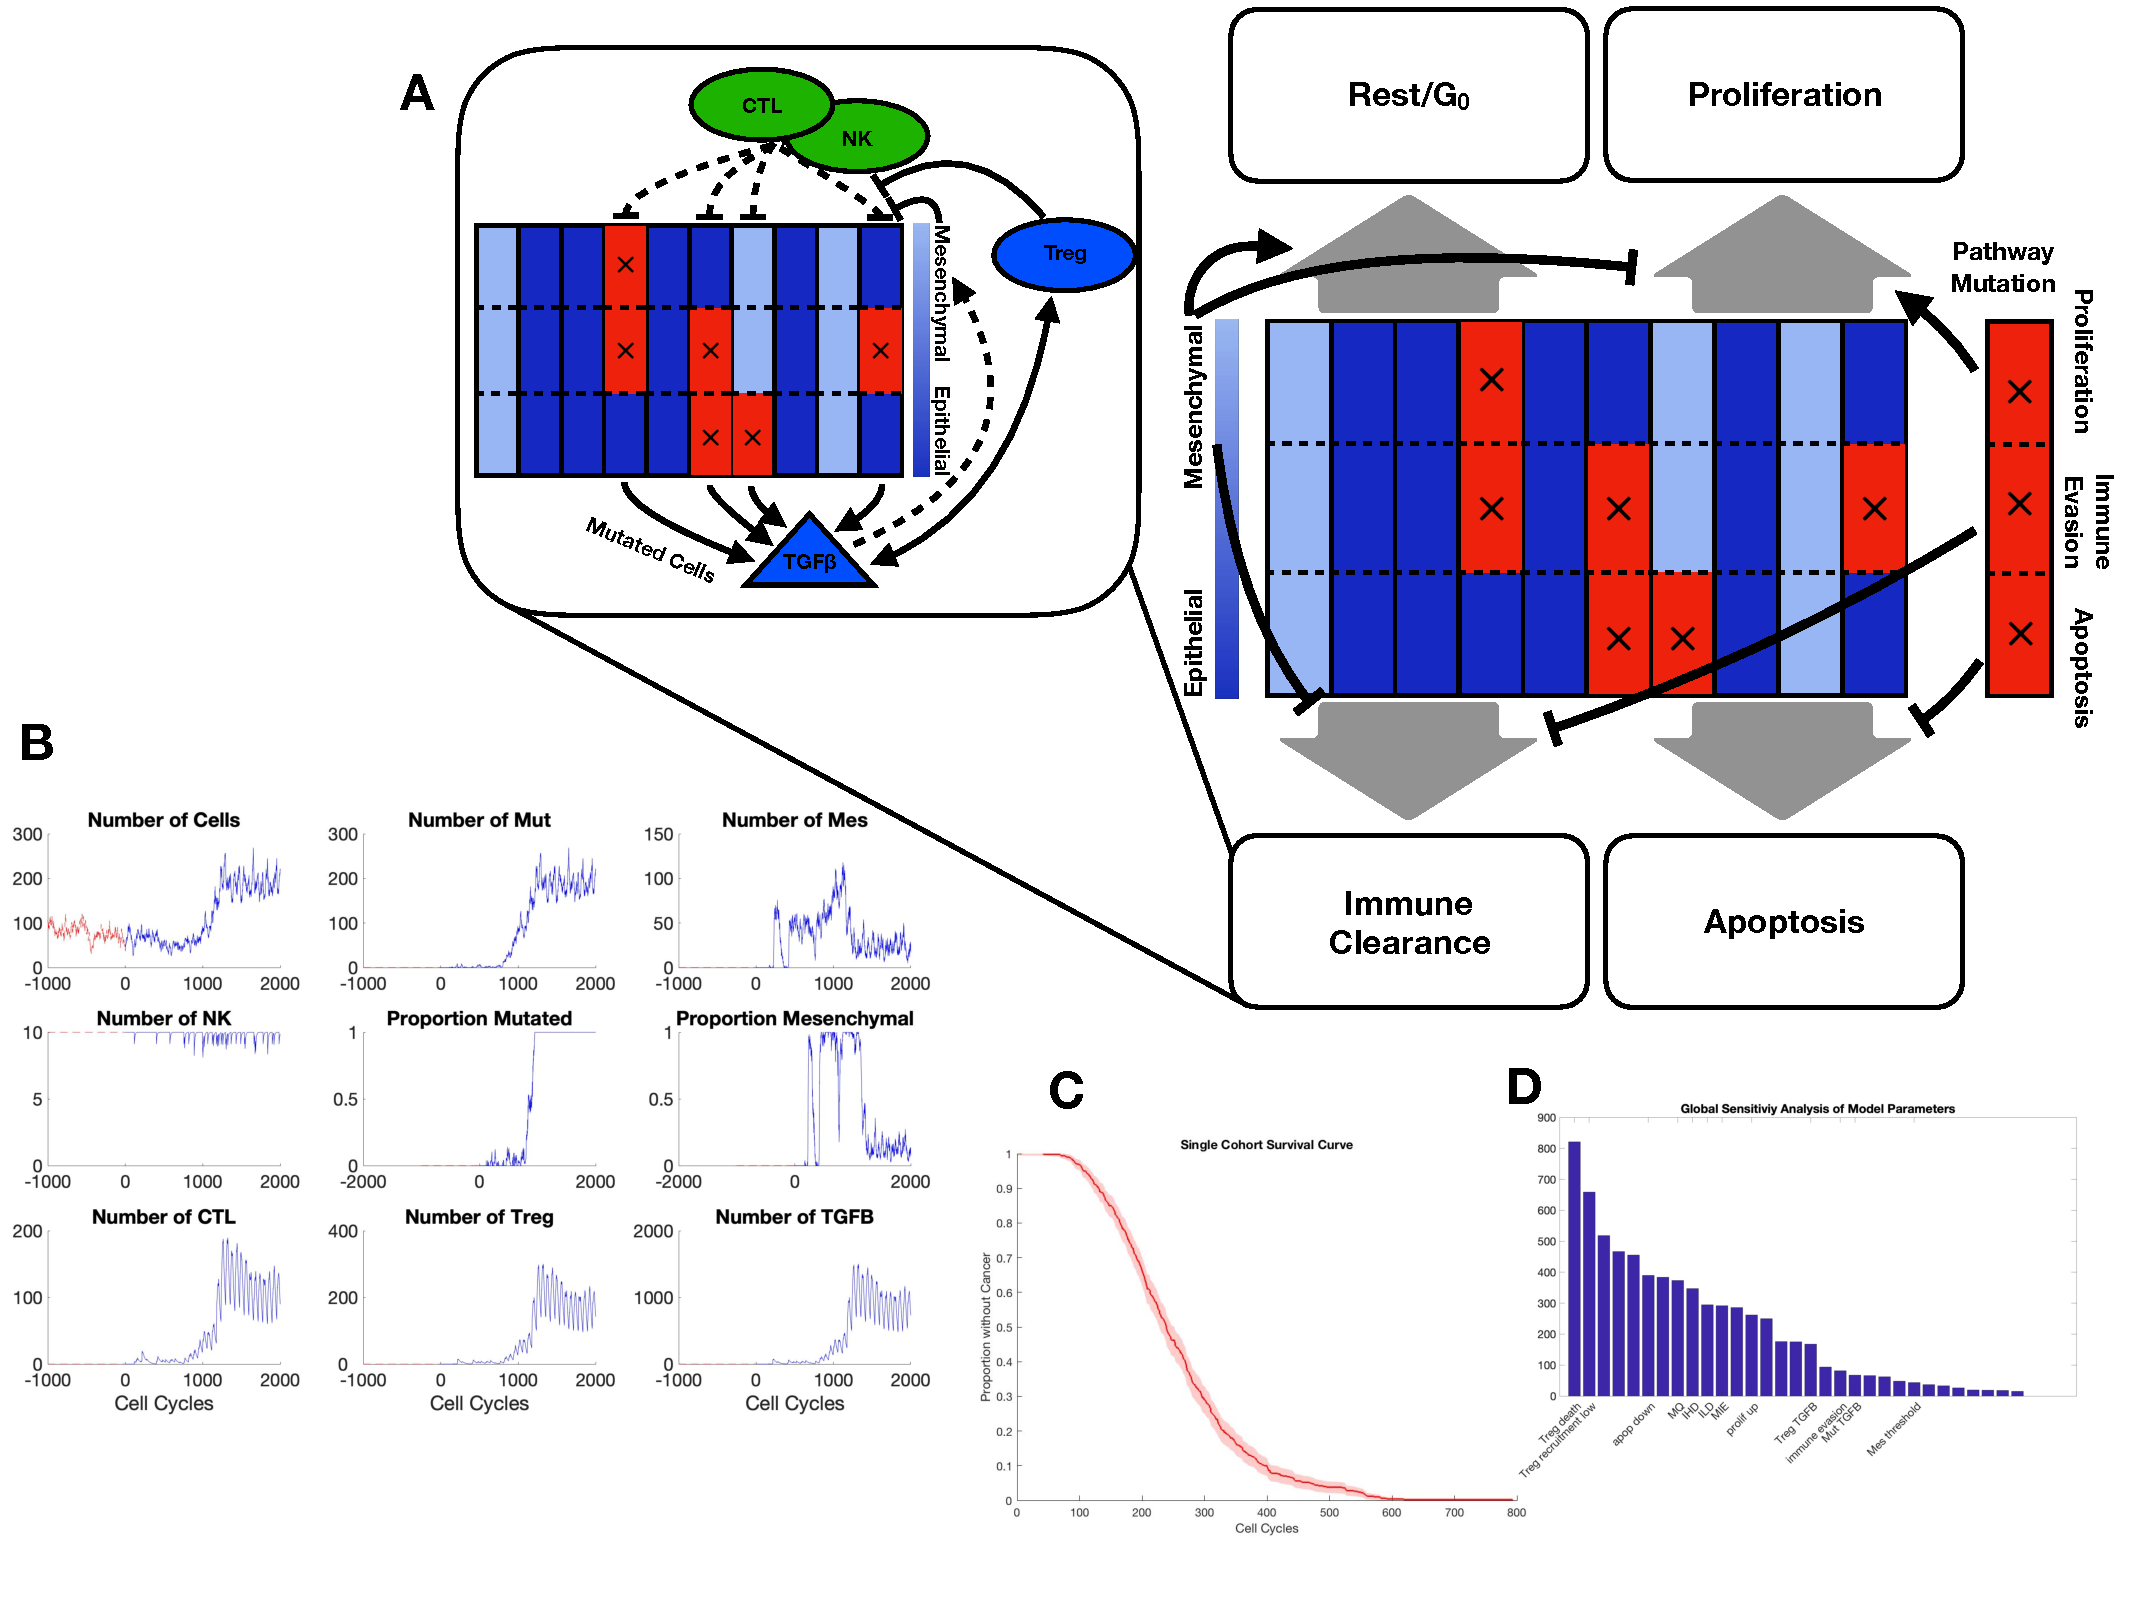
\includegraphics[width=0.8\textwidth]{Figure1/Figure1.pdf}}
\caption{A. Schematic depiction of the model with blue/red denoting non-mutated/mutated cells in the agent-based model. In each cycle, the fate of a cell is regulated by the EMT state of the cell and by any pathway mutations harbored. Inset shows major processes of immune system regulation on the tissue cells. The parameters used in this model can be found in the Supplementary material. Unless otherwise stated, parameter values are assumed to be those found in the Supplement. \tcr{Thoughts on the wording here? Once I have the table, I will use the name of that table.}
B. Example simulation of the dynamics of a one patient; warmup period is shown in red.
The inflammation cycling scheme is graphically represented above the patient dynamics.
C. Example survival curve for one cohort of patients with basal parameter values.
%A Should I list out all parameter values? A subset? Or refer to supplement for base parameter values?
D. Global sensitivity analysis of model parameters using the Morris one-step-at-a-time method.}
\label{fig:ModelIntro}
\end{figure}

We begin by investigating general features of the model to establish baseline conditions and to assess the impact of various model components on the key measured outcomes: the probability of cancer, and the Time to Cancer. 
Within the cell cycle, cell fate is determined via a set of rules that are influenced by EMT and immune interactions (Fig. \ref{fig:ModelIntro}A). For example, if a cell undergoes EMT, the probability that is will proliferate is reduced; if a cell gains a mutation in the apoptosis pathway, the probability that it undergoes apoptosis is greatly reduced. The different means by which the immune system acts on tissue cells are also shown (\ref{fig:ModelIntro}A Inset). NK cells and CTLs attempt to clear mutated tissue cells, and deactivate upon successfully carrying out their cytotoxic function. T regulatory cells (Tregs) inhibit cytotoxic activity. Tregs also release TGF-$\beta$ which promotes the recruitment of Tregs, as well as increasing the rate of EMT.
\par
The inflammation cycling scheme for a typical {\it in silico} patient consists of alternating high and low regimes (Fig. \ref{fig:ModelIntro}B); the inflammation schemes modeled will be discussed in detail in the next section. For this patient, after the warmup period, cell mutations are observed at a rate low enough that they are cleared by cytotoxic cells before being able to establish a tumor. However, after approximately 1000 cell cycles (750 days), one mutated cell exhibits clonal growth, and a tumor is established. At this point, large numbers of cells from the adaptive immune system (CTLs and Tregs) are being heavily recruited, and a peak in TGF-$\beta$ expression is observed. The number of mesenchymal cells increases initially with increasing TGF-$\beta$, but decreases after the clone takes over the tissue. This shifts back towards an epithelial tissue phenotype occurs even though the expression of TGF-$\beta$ remains high.
After 841 cell cycles, the proportion of mutated cells reaches 50\%: this is modeled as the threshold defining tumorigenesis. Thus this patient has a Time to Cancer of 841 cell cycles, or 631 days. 
After cancer incidence, the number of mutated cells continues to grow rapidly and soon makes up 100\% of the cell population. A peak in mesenchymal phenotypes is observed following cancer incidence, before most transition back to an epithelial state.
\par 
Considering the immune system dynamics, we see that the NK population is approximately constant, while the adaptive populations (CTL and Treg cells) grow quickly and dwarf NK cells in number following the accumulation of oncogenic mutations.
%Note: NK cells also lymphocytes! 
The adaptive immune populations also exhibit oscillatory behavior, however note that this is not due to intrinsic dynamics but rather due to the inflammation scheme that the patient is undergoing: alternating between 30 cell cycles of high inflammation and 60 cell cycles of low inflammation. Within each of these periods, adaptive immune populations increase or decrease rapidly in accordance with the inflammation state.
\par 
The {\em in silico} patient described here is given for the purpose of illustrating features the model. Given the multiple sources of noise in the model, in order to quantify patient dynamics and cancer-free survival rates, below we will simulate large cohorts of patients. In Fig. \ref{fig:ModelIntro}C we simulate the survival curve for a cohort of $500$ patients: we see that all the patients survive for approximately 100 cell cycles (75 days). Subsequently, in the approximate range of $T= [100,300]$, the cancer onset rate is roughly constant, and after $600$ cell cycles, no patients remain cancer free.


\subsection{Identification of key regulatory parameters via Morris global sensitivity analysis}\label{SensAnalysis}
To assess the sensitivity of the model parameters and thus identify those that are most important in determining cancer-free survival times, we applied Morris one-step-at-a-time (OAT) sensitivity analysis (see Methods) to the model.
% Sentence on how it is 'global' and sentence on what the measured output is (ie y axis) 
...
The results of Morris OAT on the 31 model parameters are shown in \ref{fig:MOAT}: a subset of parameters demonstrate much higher levels of sensitivity than others.
The two most influential according to this analysis are the death rate and the recruitment rate of Treg cells, this is most likely due to the dual roles Treg cells play in both suppressing the cytotoxic effects of other immune cells and secreting TGF-$\beta$, which drives EMT.
This ties Treg cells to all three components of the model.
Since we seek to separate the effects of different model components, we do not choose the parameters influencing Treg cells for detailed analysis below.
\par
%% We need to discuss parameter names. Maybe replace 'low' with 'base' and 'up' with 'gain' ?
Any of the parameters in the \tcr{table} which include the word ``low'' are parameters that govern the model in a low inflammatory state.
With the exception of ``prolif up'', all parameters that end in ``up'' or have `U' at the end of their abbreviation, are the factors by which these parameters change when the system switches from low to high inflammation.
The IHD and ILD parameters determine the duration of high and low inflammation, respectively.
A cell with mutated pathways will be affected by the ``apop down'', ``prolif up'', and ``immune evasion'' parameters, depending on which pathways are mutated.
The mesenchymal cells are influenced by the MGA and MIE parameters.
Finally, $\sigma$, $k_\text{EMT}$, TGFB$_{max}$, and $\gamma_\text{EC50}$ all control how cells transition between the epithelial and mesenchymal states.

Since one goal of our analysis is to assess the specific effects of EMT on immune-cancer dynamics, the parameters MIE and MGA are of particular interest.
In addition, inflammation parameters dictating the cycling scheme are important to study\tcr{REF}: we find that there are also high sensitivities in this model to these parameters.
In terms of Treg cells, their secretion of TGF-$\beta$ is highly significant and we will also study it further.


\begin{figure}
\center
{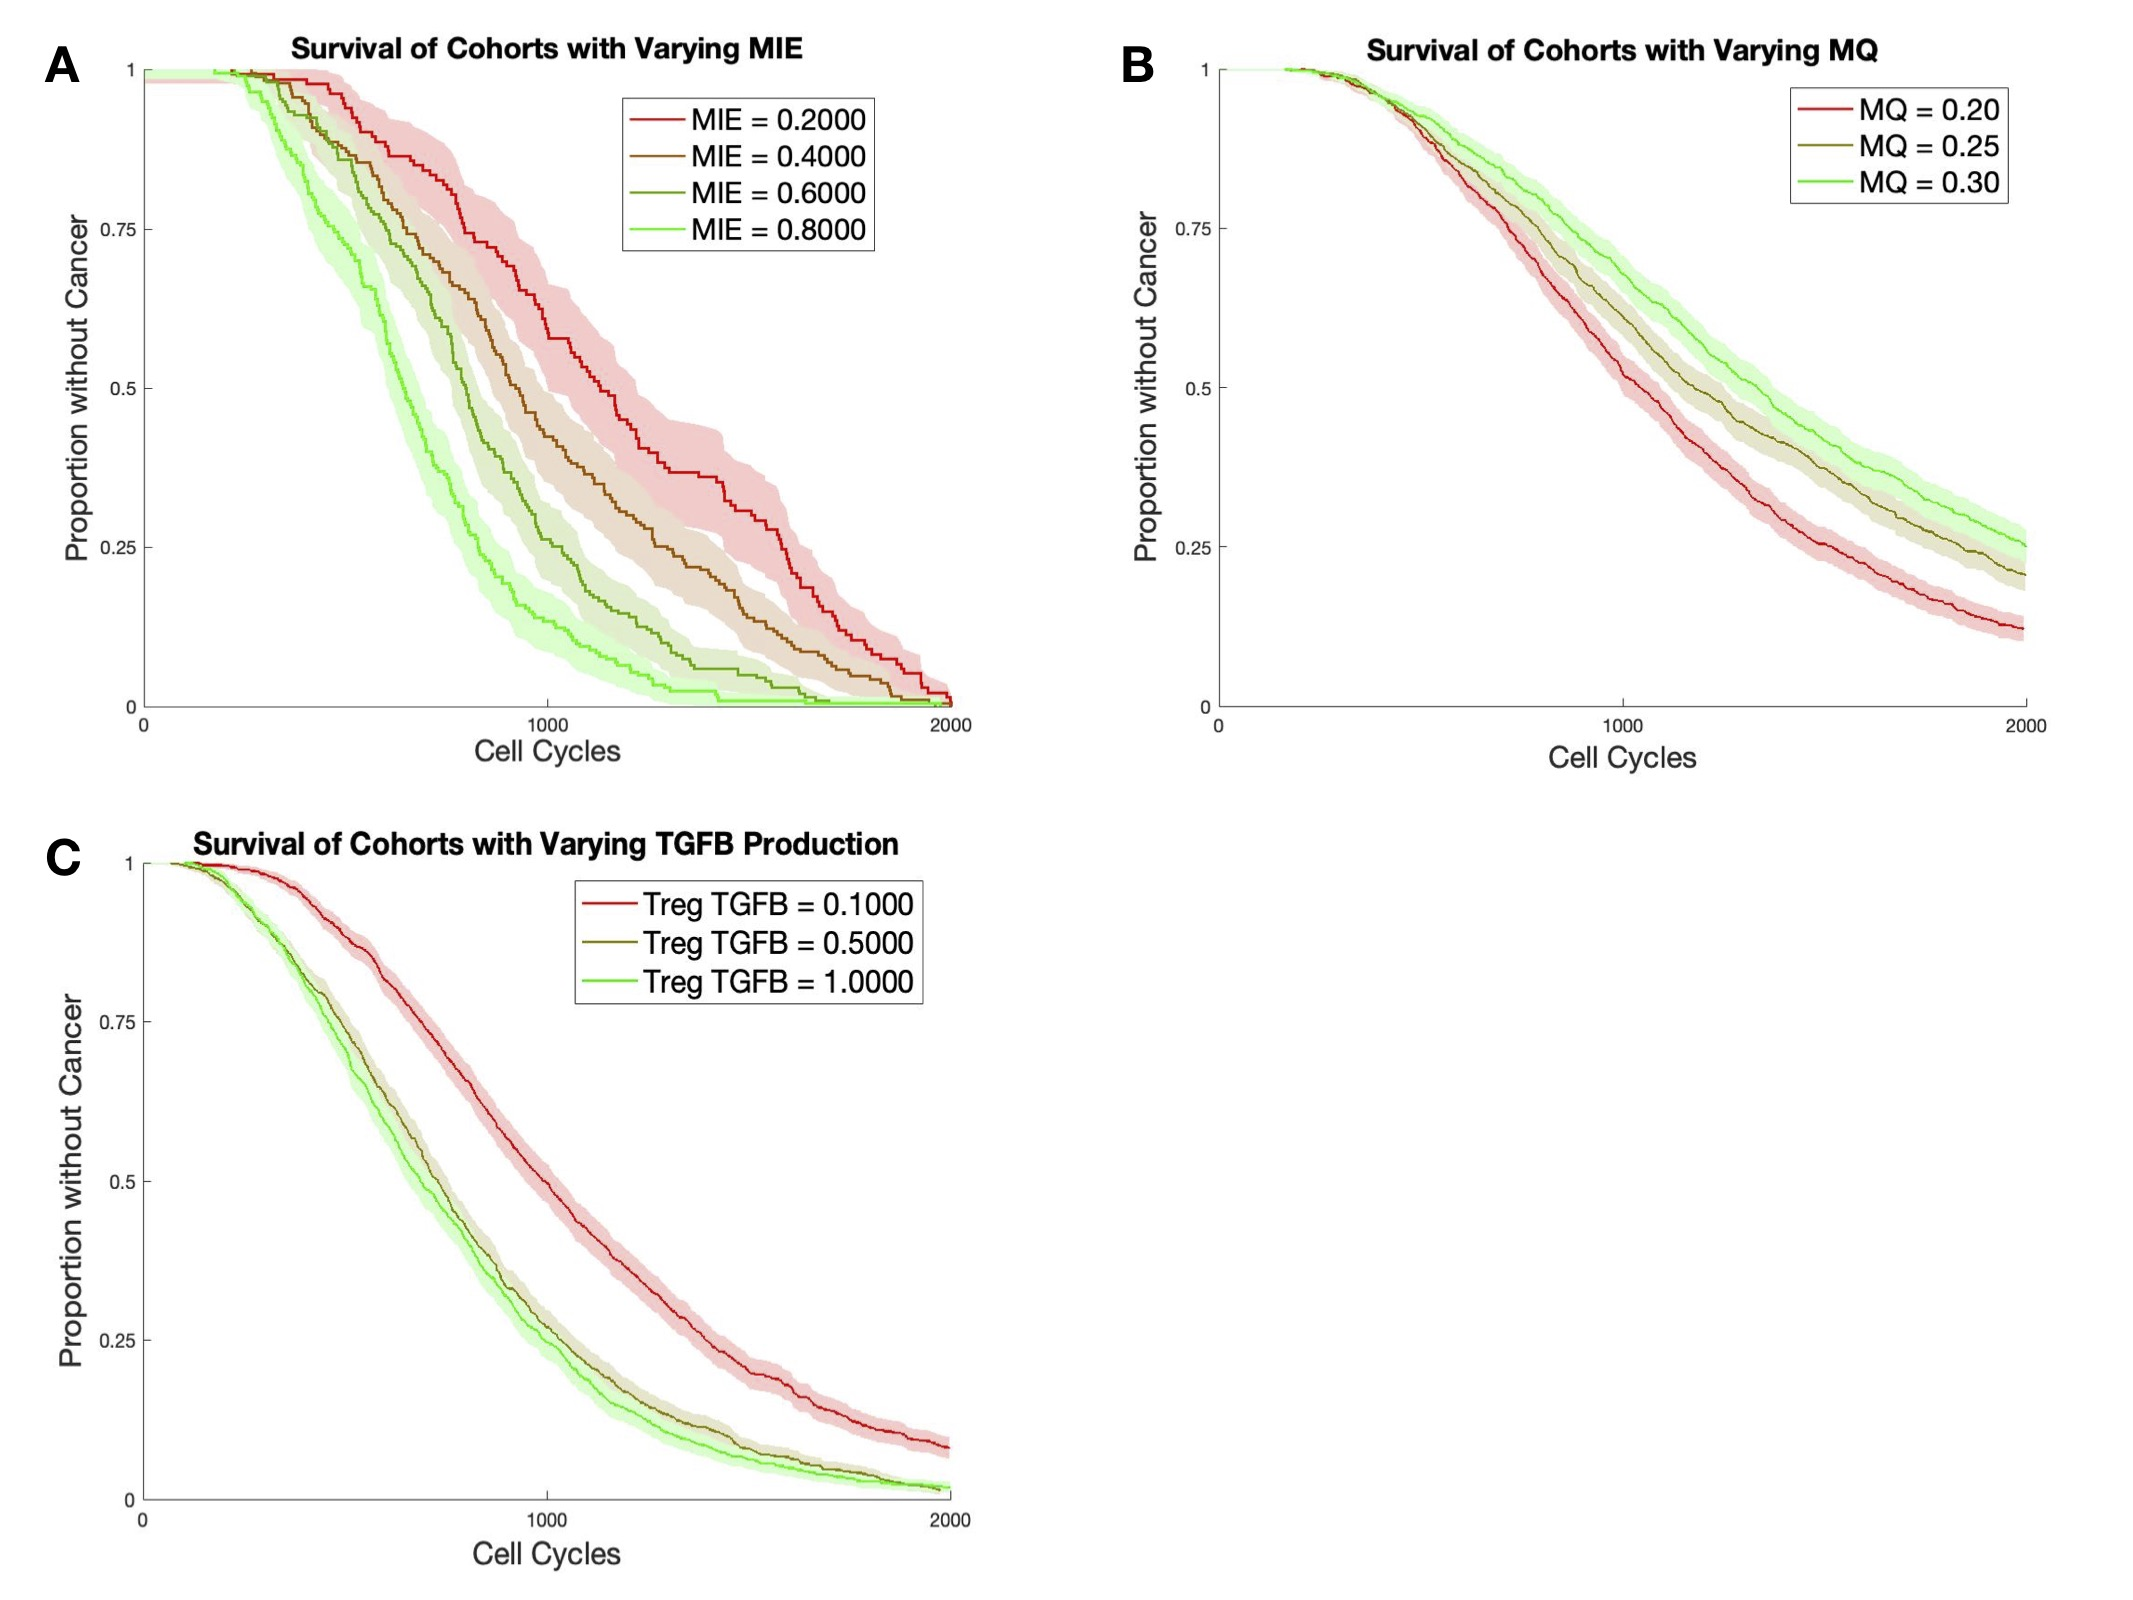
\includegraphics[width=0.85\textwidth]{Figure2/Figure2.jpg}}
\caption{Global sensitivity analysis of model parameters using the Morris one-step-at-a-time method.}
\label{fig:MOAT}
\end{figure}




\subsection{Mesenchymal phenotypic properties dramatically change cancer-free survival times}\label{MesPars}

\begin{figure}
\center
{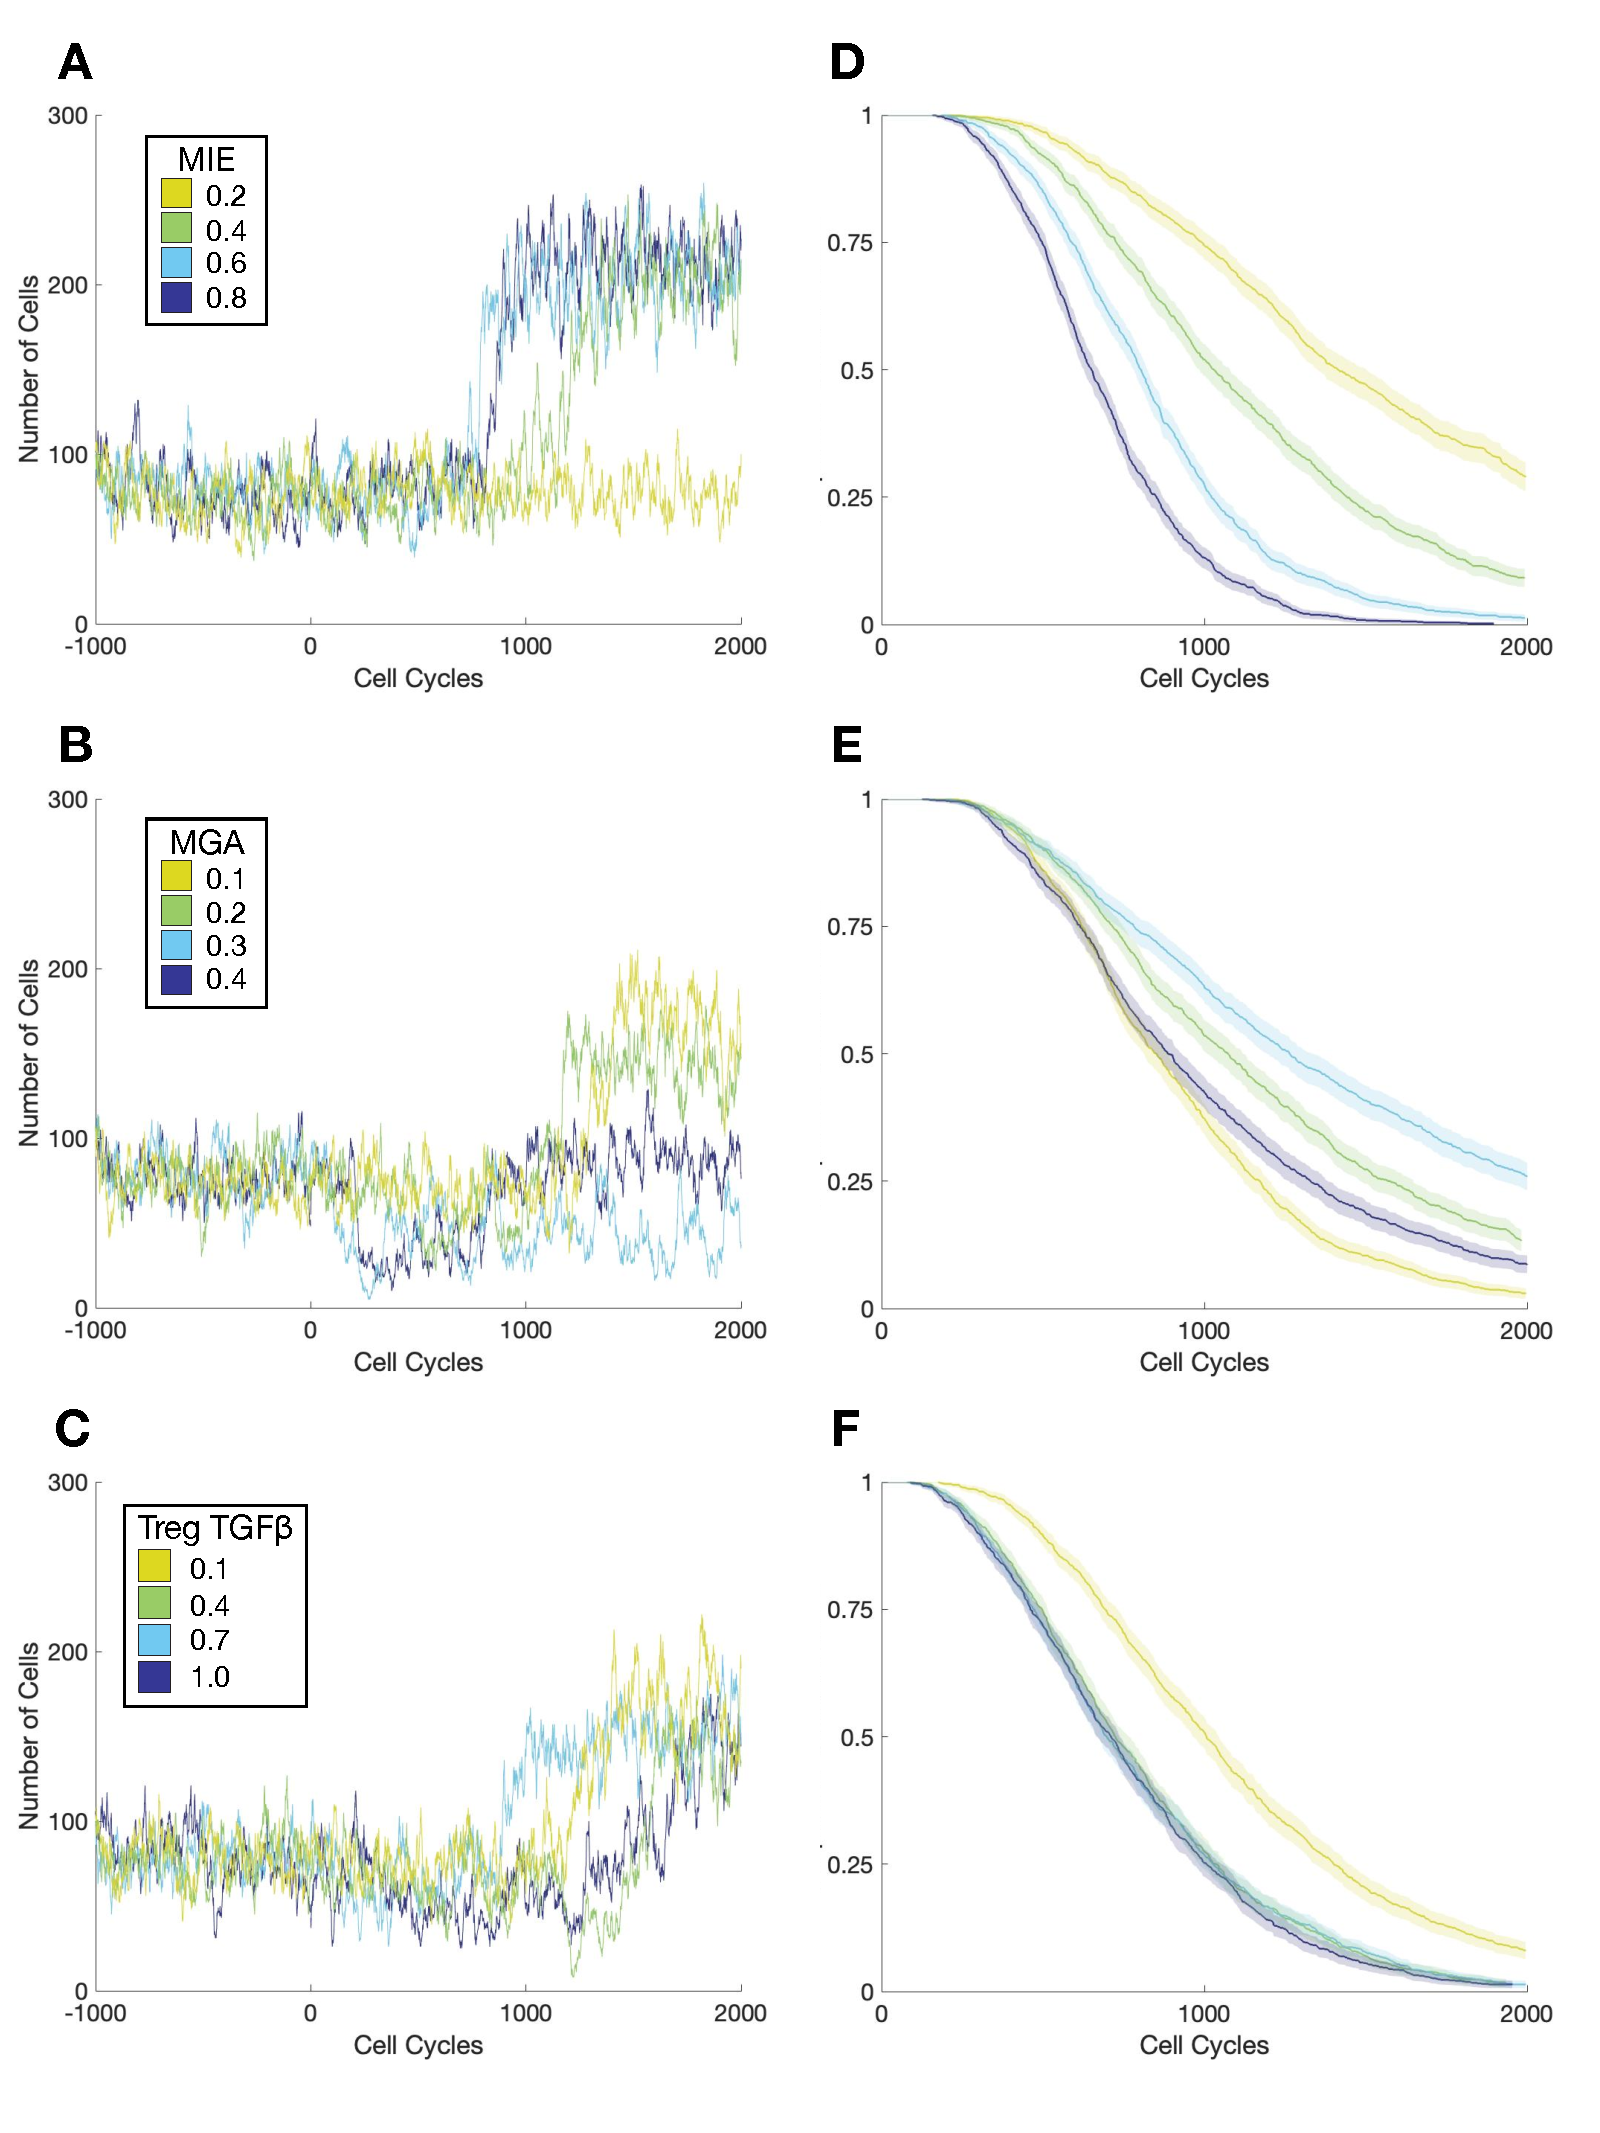
\includegraphics[width=0.85\textwidth]{Figure3/Figure3.pdf}}
\caption{
A-C. Trajectory of one patient per cohort followed from warmup through 2000 cell cycles while varying MIE (A), MGA (B) or XXXXXX (C). 
D. Increasing MIE decreases Time to Cancer. 
E. Increasing MGA increases Time to Cancer.
F. Increasing Treg TGF-$\beta$ production results in decreased Time to Cancer.
%% \color{red} Cox regression or KM test statistics to be computed to demonstrate the significance of this claim.
}
\label{fig:FirstSurvivalCurves}
\end{figure}


When a cell transitions from an epithelial to a mesenchymal state, two phenotypic cell characteristics change: mesenchymal immune evasion (MIE) and mesenchymal growth arrest (MGA).
Both parameters are defined as proportions, and lie in $[0,1]$, where higher values indicate more mesenchymal-like properties.
MIE is the proportional reduction in the probability that a mutated mesenchymal cell will be subject to immune clearance in a given cycle.
MGA is the proportional reduction in the probability that a mesenchymal cell will proliferate in a given cell cycle, thus is equivalent (strictly in terms of its impact on the cell cycle) to an increased proportion of time spent resting in the $G_0$ phase.
The cytokine TGF-$\beta$ is also involved in the EMT process (by increases the probability of EMT). All three of these parameters were found to have large effects on the model by the Morris OAT analysis presented in Section \ref{SensAnalysis}.
\par 
As the level of mesenchymal immune evasion (MIE) is increased, the Time to Cancer decreases (Fig. \ref{fig:FirstSurvivalCurves}A) under all sets of parameters studied: as this subpopulation of potentially mutated cells becomes more resistant to immune clearance, the tumor as a whole grows more resilient and thus will grow faster.
These results are summarized by Figure \ref{fig:FirstSurvivalCurves}A.

Second, as the rate of mesenchymal growth arrest (MGA) increases, Time to Cancer increases, i.e. lower proliferation rates for mesenchymal cells slow down cancer growth (Figure \ref{fig:FirstSurvivalCurves}B).
This is not immediately intuitive, since the decreased proliferation rate affects both mutated and non-mutated tissue cells.

Third, TGF-$\beta$ can be varied in two ways: the production by mesenchymal cells and the production by Treg cells.
In Figure \ref{fig:FirstSurvivalCurves}C, the results of varying Treg TGF-$\beta$ production are shown, indicating that an increased Treg TGF-$\beta$ production leads to a shorter Time to Cancer.
The two main ways in which TGF-$\beta$ influences the system is in recruitment of Treg cells and in pushing tissue cells to a mesenchymal phenotype.
Treg cells are modeled as tumor-protective and thus increasing their number will naturally decrease Time to Cancer.
Mesenchymal cells are more likely to evade the immune system, so pushing the system towards an overall more mesenchymal phenotype will better protect the cancer and decrease the Time to Cancer.



\subsection{A key EMT regime maximizes cancer-free survival time under chronic inflammation}\label{KeyEMT}

We explored the effects of varying the inflammation state of the patient on cancer-free survival, to investigate competing interactions within the TME and their effect on EMT. Patient cohorts were simulated under different inflammation regimes: permanently low inflammation; permanently high inflammation; or variable inflammatory. For patients drawn from cohorts in a permanently high inflammatory state, the relationship between mesenchymal parameters and the Time to Cancer is monotonic, i.e. increasing either the rate of mesenchymal immune evasion (MIE) (Fig. \ref{fig:VaryINFL_and_MesPars}A-B) or of mesenchymal growth arrest (MGA)  (Fig. \ref{fig:VaryINFL_and_MesPars}C-D) decreases the Time to Cancer.
However, under regimes with either temporary or permanent periods of low inflammation, different relationships emerge: a local maximum for the Time to Cancer is found with respect to the relative mesenchymal growth rate (MGA $= 0.3$). This is seen both for intermittent or low inflammation (Fig. \ref{fig:VaryINFL_and_MesPars}D). 
\par
These striking differences in the mean Time to Cancer -- extended by up to one year by fine-grained optimization of mesenchymal growth arrest -- have clear therapeutic implications. 
%What this indicates is that if the growth arrest of mesenchymal cells can be controlled, then they could be manipulated in such a way as to increase the Time to Cancer.
%For patients presenting with chronically high inflammatory state, anti-inflammatories could be administered which would create the periods of low inflammation our model predicts as necessary for seeing these changes.
Our model predicts that reducing the inflammatory state of the TME in three weeks out of every nine would be provide means to prolong cancer-free survival in combination with mesenchymal cell therapies to make the control of mesenchymal proliferation an effective anti-cancer strategy.
\par
In contrast, when MIE is varied for different inflammation cycling schemes, regardless of the cycling scheme, increasing the MIE leads to decreases in the Time to Cancer (worse survival probabilities), although in the case where the inflammatory state is permanently high, MIE has little effect on the Time to Cancer. Thus under any inflammation regime with periods of low inflammation, any reductions in the rate of mesenchymal immune evasion will lead to improved patient outcomes.

\begin{figure}
\center
{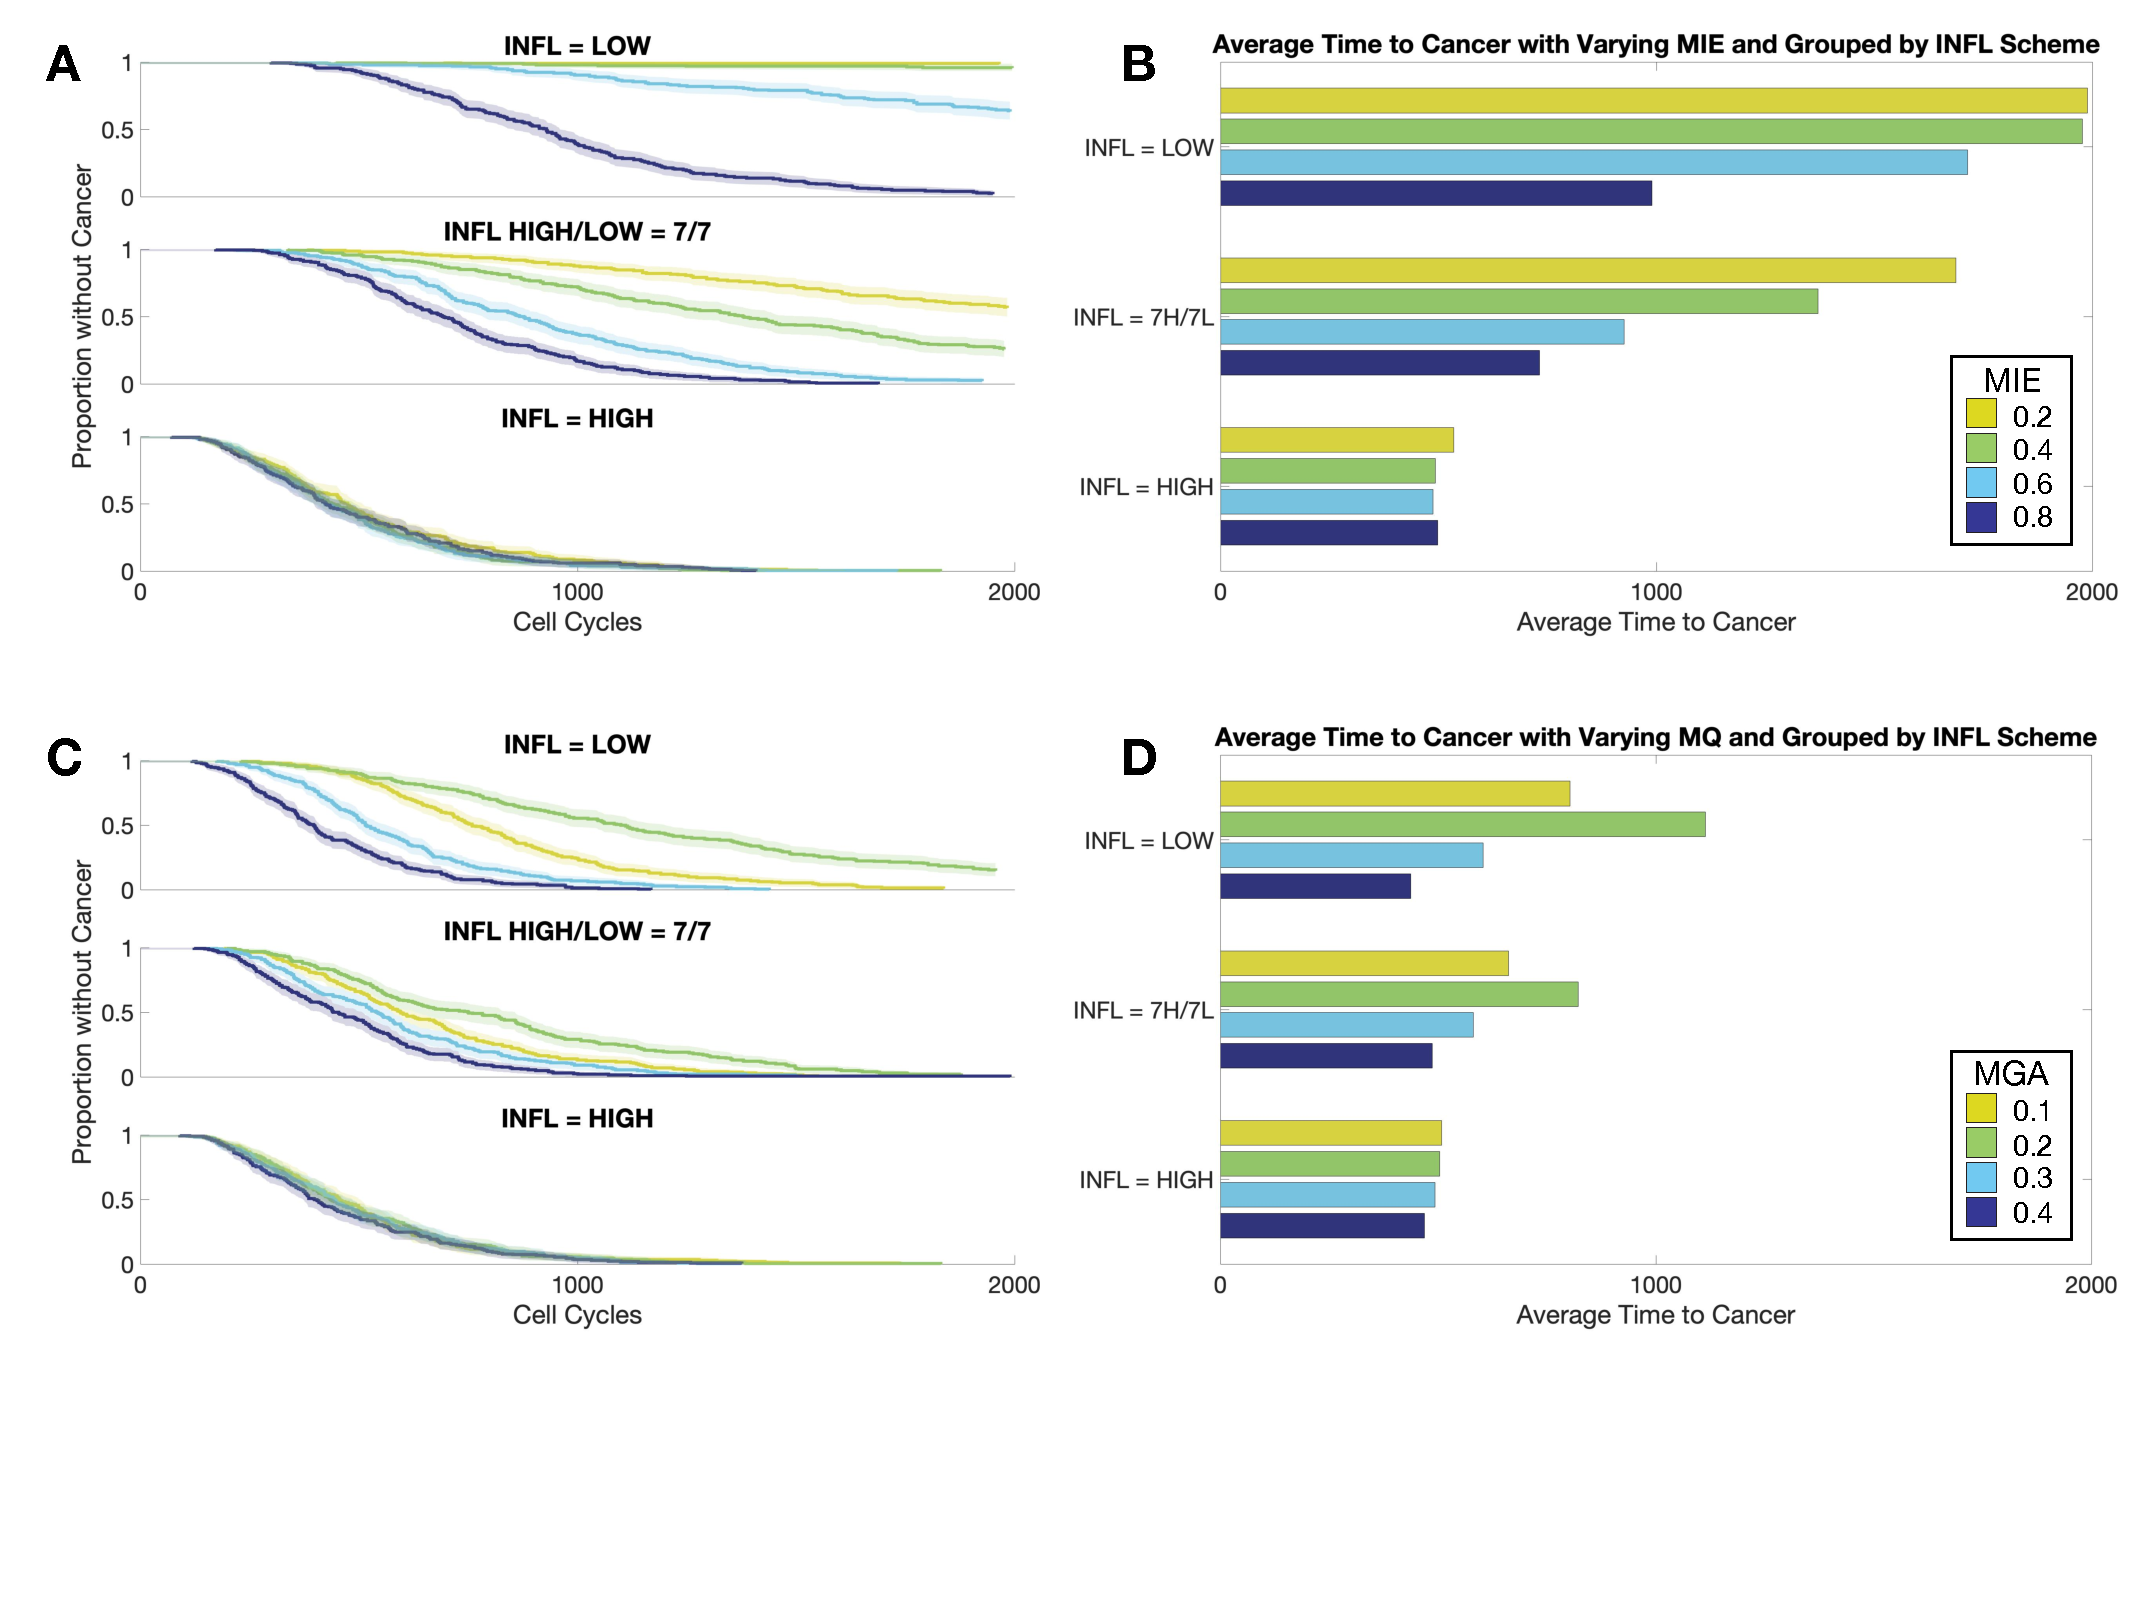
\includegraphics[width=0.9\textwidth]{Figure4/Figure4.pdf}}
\caption{A. Survival curves for various inflammation cycling schemes. In the top two plots, the Time to Cancer decreases as MIE increases. In the bottom plot, there is no significant difference in survival.
B. The average Time to Cancer for each cohort.
C. Survival curves for various inflammation cycling schemes. In the top two plots, the Time to Cancer reaches a maximum value somewhere near MGA = 0.3. In the bottom plot, there is no significant difference in survival.
D. The average Time to Cancer for each cohort.}
\label{fig:VaryINFL_and_MesPars}
\end{figure}


\begin{figure}
\center
{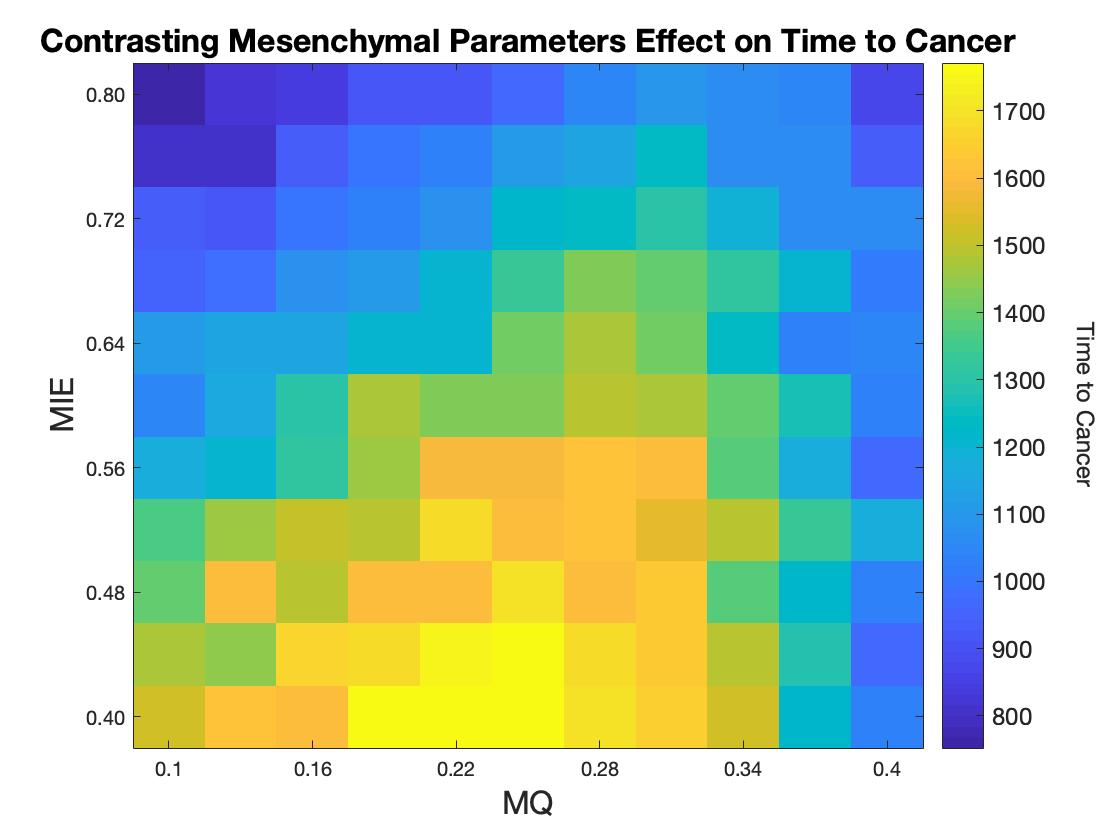
\includegraphics[width=0.6\textwidth]{Figure5/MIEvsMQ.jpg}}
\caption{Heat Map contrasting the effects of MIE and MGA on Time to Cancer. Increasing MIE always decreases Time to Cancer, but MGA is non-monotonically linked to Time to Cancer.}
\label{fig:MIEvsMGA}
\end{figure}


% \subsection{Heat Map of MIE vs MGA}
\subsection{Analysis of TCGA data in comparison with model predictions suggests that mesenchymal phenotypes reduce cancer-free survival probability}\label{tcga}

To further assess the effects on tumorigenesis of the mesenchymal properties of immune evasion (MIE) and growth arrest (MGA), we study the joint density plot for each of these parameters against the Time to Cancer (Fig. \ref{fig:MIEvsMGA}). We found that over the full range of values of MGA considered, increasing the MIE decreases the Time to Cancer. However, for any given value of mesenchymal immune evasion, there is a value of mesenchymal growth arrest that maximizes the Time to Cancer. Moreover, this optimal value increases with increasing MIE. Together these results show that while reducing the ability of a mutated cell to evade the immune system by any amount will improve the probability of cancer-free survival, an optimal value of MGA will prolong survival. 
\par 
To compare these model predictions with experimental studies, we analyzed data from The Cancer Genome Atlas (TCGA) database to study the effects of immune and EMT interactions on prognosis of cancers for which inflammation is known to play an important role, such as colonic or pancreatic cancers \cite{hu10_inflammationinduced, balkwill01_inflammation}. Using gene ontologies as a measure of the of effects of inflammatory or EMT processes on cancer-free survival, we investigate pancreatic cancer. We note that the comparison between simulation and data here is indirect since the model studies processes occurring before incidence, while the data address subsequent events, but analogous processes are at play during both the pre-cancerous clonal dynamics addressed by the model, and the progression of disease that follows cancer incidence. 
\par
For a cohort of pancreatic cancer patients, we cluster the patients via k-means ($n=2$) either on gene ontologies relating only to EMT (Fig. \ref{fig:tcga}A) or on gene ontologies relating to EMT and inflammation (Fig. \ref{fig:tcga}C). We also plot the corresponding survival curves for each of the clusters obtained (Fig. \ref{fig:tcga}B, D). We see that in both cases, survival is significantly affected by the gene ontology signature, but, importantly, the presence of both EMT and inflammatory signatures has a greater impact on survival than the effects of EMT alone. This suggests that 


\begin{figure}
\center
{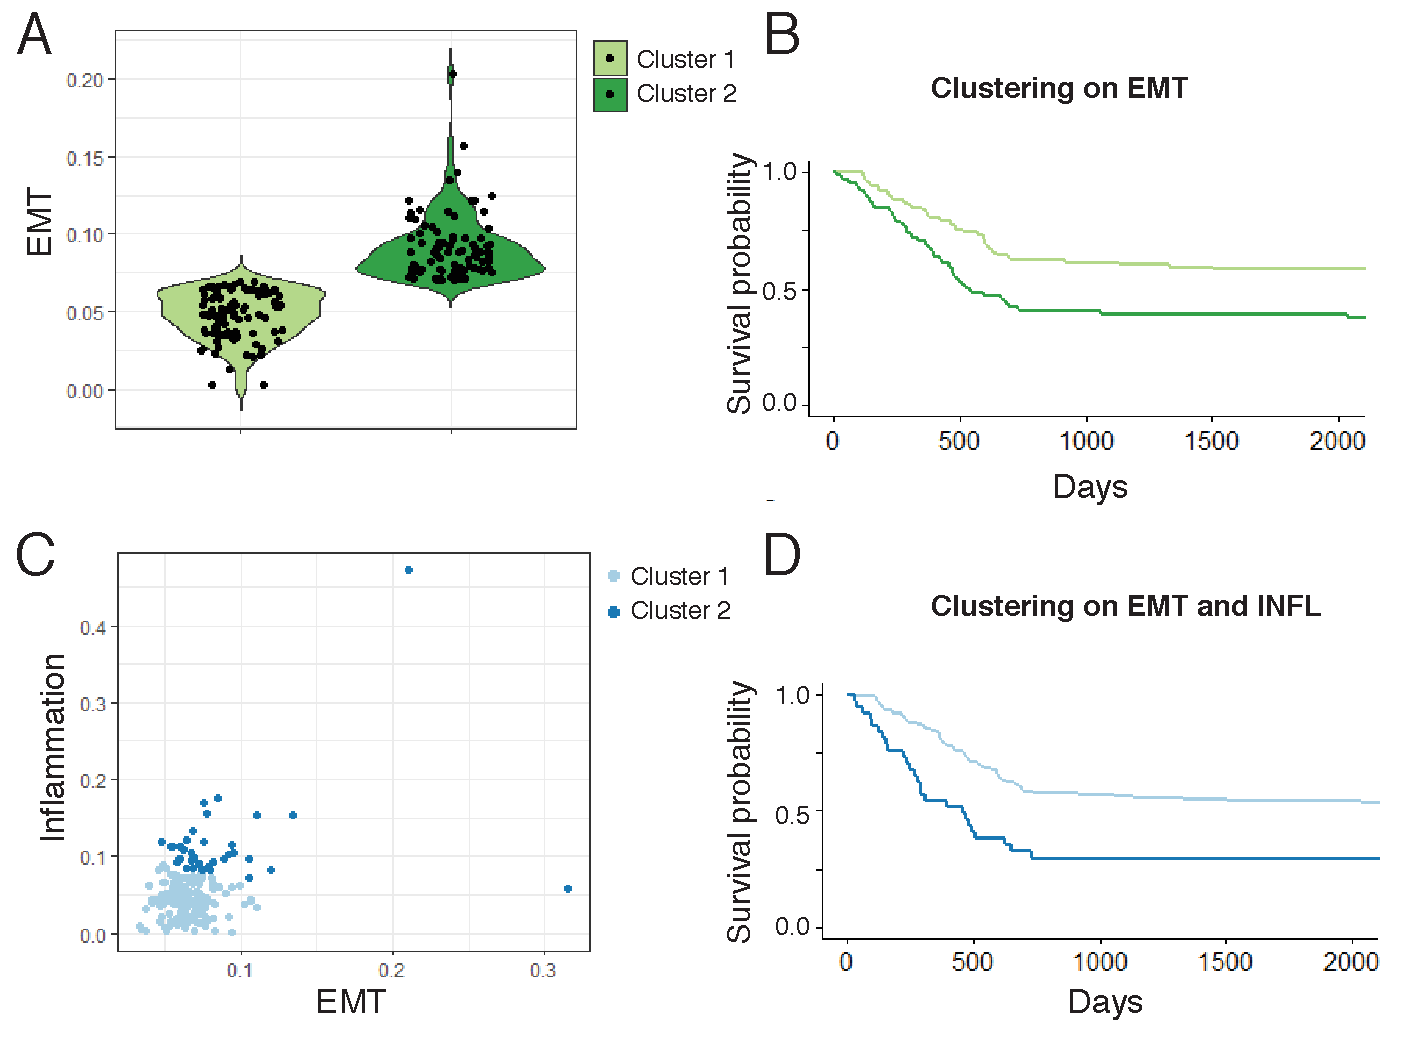
\includegraphics[width=\columnwidth]{FigTCGA.pdf}}
\caption{A. K-means clustering of pancreatic cancers using gene ontology terms indicative of an EMT signature ($k=2$). B. Survival plots corresponding to the clustering on EMT. C. K-means clustering of pancreatic cancers using gene ontology terms indicative of EMT and Inflammation signatures ($k=2$). D. Survival plots corresponding to the clustering on EMT and inflammation.}
\label{fig:tcga}
\end{figure}



%%%%%%%%%%%%%%%%%%%%%%%
%                      DISCUSSION                       %
%%%%%%%%%%%%%%%%%%%%%%%

\section{Discussion}\label{Discussion}
In building this model, we set out to better understand how the immune system and the EMT spectrum would affect Time to Cancer results from previous work.
What we found is that altering many of the processes have predictable results: increasing mesenchymal immune evasion, decreasing mesenchymal growth arrest, and increasing Treg TGF-$\beta$ production all lead to shorter Times to Cancer.
However, when the inflammation of the TME is accounted for, some of these changes to the system have less predictable outcomes.
The most intriguing is that periods of low inflammation lead to mesenchymal growth arrest having an optimal value for maximizing Time to Cancer.



%In addition, I could discuss the implications from the TGF-$\beta$ section.
%Any discussion on this topic, however, would need to acknowledge that regulation of TGF-$\beta$ might also have other, serious side effects, especially if the treatment is not local.
%However, that might also be true for the inflammatory results.
%In light of this, it might be good to include a new section on how TGF-$\beta$ production's influence on Time to Cancer is influenced by the inflammatory cycling scheme.


%% AM: no need to separate this I think - combine conclusions into the discussion section. 
%\section{Conclusion}\label{Conclusion}
The interactions of the immune system and cancer remain a promising avenue of research.
Including more diverse aspects of the TME and the tumor itself make the challenge that much harder but also that much more promising.
As we begin to understand how processes such as EMT factor in to these complex interactions, we can begin to respond clinically to better improve patient outcomes.
Here, we saw {\it in silico} evidence of an optimal value for a property of mesenchymal cells that would maximize Time to Cancer.
There is still much work to be done further isolating this effect in computer simulations and further verifying this effect and exploring further ways EMT can influence tumor progression.
This model explored much more than mesenchymal growth arrest, so a simpler model could make this point clearer.
On the other hand, models which incorporate more distinctions between epithelial and mesenchymal cells could give better clarity on the relative importance of these and reveal a fuller picture about how a mesenchymal subpopulation affects cancer outcomes.

%A Adam, do you know of any?
The authors are not aware of current treatments that specifically target mesenchymal growth arrest, influencing it in one direction or another.
%
Based on these results, this could prove to be a promising direction for research, in particular for cancers in which it is known that mesenchymal cells are present and active within the tumor.
The greatest challenge in translating the information here to the clinic, apart from creating the drugs, would be discovering the ideal growth rate for mesenchymal cells within each patient and how other patient-specific data will influence this result.

Progress in cancer treatment has always proven attainable even despite great challenges, for which the complexity of the disease is often responsible. As we move forwards, it is these very complexities that we will be able to better exploit to eradicate or control the disease.


\section*{Acknowledgements}

\bibliography{mybib,amrefs}
\bibliographystyle{plos2015}

\end{document}